\documentclass[addpoints, 12pt]{exam}%, answers]
\usepackage[utf8]{inputenc}
\usepackage[T1]{fontenc}

\usepackage{lmodern}
\usepackage{arydshln}
\usepackage[margin=2cm]{geometry}

\usepackage{enumitem}

\usepackage{amsmath, amsthm, amsfonts, amssymb}
\usepackage{graphicx}
\usepackage{tikz}
\usetikzlibrary{arrows,calc,patterns}
\usepackage{pgfplots}
\pgfplotsset{compat=newest}
\usepackage{url}
\usepackage{multicol}
\usepackage{thmtools}
\usepackage{wrapfig}

\usepackage{caption}
\usepackage{subcaption}

\usepackage{pifont}

% MATH commands
\newcommand{\bC}{\mathbb{C}}
\newcommand{\bR}{\mathbb{R}}
\newcommand{\bN}{\mathbb{N}}
\newcommand{\bZ}{\mathbb{Z}}
\newcommand{\bT}{\mathbb{T}}
\newcommand{\bD}{\mathbb{D}}

\newcommand{\cL}{\mathcal{L}}
\newcommand{\cM}{\mathcal{M}}
\newcommand{\cP}{\mathcal{P}}
\newcommand{\cH}{\mathcal{H}}
\newcommand{\cB}{\mathcal{B}}
\newcommand{\cK}{\mathcal{K}}
\newcommand{\cJ}{\mathcal{J}}
\newcommand{\cU}{\mathcal{U}}
\newcommand{\cO}{\mathcal{O}}
\newcommand{\cA}{\mathcal{A}}
\newcommand{\cC}{\mathcal{C}}
\newcommand{\cF}{\mathcal{F}}

\newcommand{\fK}{\mathfrak{K}}
\newcommand{\fM}{\mathfrak{M}}

\newcommand{\ga}{\left\langle}
\newcommand{\da}{\right\rangle}
\newcommand{\oa}{\left\lbrace}
\newcommand{\fa}{\right\rbrace}
\newcommand{\oc}{\left[}
\newcommand{\fc}{\right]}
\newcommand{\op}{\left(}
\newcommand{\fp}{\right)}

\newcommand{\ra}{\rightarrow}
\newcommand{\Ra}{\Rightarrow}

\renewcommand{\Re}{\mathrm{Re}\,}
\renewcommand{\Im}{\mathrm{Im}\,}
\newcommand{\Arg}{\mathrm{Arg}\,}
\newcommand{\Arctan}{\mathrm{Arctan}\,}
\newcommand{\sech}{\mathrm{sech}\,}
\newcommand{\csch}{\mathrm{csch}\,}
\newcommand{\Log}{\mathrm{Log}\,}
\newcommand{\cis}{\mathrm{cis}\,}

\newcommand{\ran}{\mathrm{ran}\,}
\newcommand{\bi}{\mathbf{i}}
\newcommand{\Sp}{\mathrm{span}\,}
\newcommand{\Inv}{\mathrm{Inv}\,}
\newcommand\smallO{
  \mathchoice
    {{\scriptstyle\mathcal{O}}}% \displaystyle
    {{\scriptstyle\mathcal{O}}}% \textstyle
    {{\scriptscriptstyle\mathcal{O}}}% \scriptstyle
    {\scalebox{.7}{$\scriptscriptstyle\mathcal{O}$}}%\scriptscriptstyle
  }
\newcommand{\HOL}{\mathrm{Hol}}
\newcommand{\cl}{\mathrm{clos}}
\newcommand{\ve}{\varepsilon}

\DeclareMathOperator{\dom}{dom}

%%%%%% Définitions Theorems and al.
%\declaretheoremstyle[preheadhook = {\vskip0.2cm}, mdframed = {linewidth = 2pt, backgroundcolor = yellow}]{myThmstyle}
%\declaretheoremstyle[preheadhook = {\vskip0.2cm}, postfoothook = {\vskip0.2cm}, mdframed = {linewidth = 1.5pt, backgroundcolor=green}]{myDefstyle}
%\declaretheoremstyle[bodyfont = \normalfont , spaceabove = 0.1cm , spacebelow = 0.25cm, qed = $\blacktriangle$]{myRemstyle}

%\declaretheorem[ style = myThmstyle, name=Th\'eor\`eme]{theorem}
%\declaretheorem[style =myThmstyle, name=Proposition]{proposition}
%\declaretheorem[style = myThmstyle, name = Corollaire]{corollary}
%\declaretheorem[style = myThmstyle, name = Lemme]{lemma}
%\declaretheorem[style = myThmstyle, name = Conjecture]{conjecture}

%\declaretheorem[style = myDefstyle, name = D\'efinition]{definition}

%\declaretheorem[style = myRemstyle, name = Remarque]{remark}
%\declaretheorem[style = myRemstyle, name = Remarques]{remarks}

\newtheorem{theorem}{Théorème}
\newtheorem{corollary}{Corollaire}
\newtheorem{lemma}{Lemme}
\newtheorem{proposition}{Proposition}
\newtheorem{conjecture}{Conjecture}

\theoremstyle{definition}

\newtheorem{definition}{Définition}[section]
\newtheorem{example}{Exemple}[section]
\newtheorem{remark}{\textcolor{red}{Remarque}}[section]
\newtheorem{exer}{\textbf{Exercice}}[section]


\tikzstyle{myboxT} = [draw=black, fill=black!0,line width = 1pt,
    rectangle, rounded corners = 0pt, inner sep=8pt, inner ysep=8pt]

\begin{document}
	\noindent \hrulefill \\
	\noindent MATH-244 \hfill Created by Pierre-O. Paris{\'e}\\
	Midterm 03 \hfill November, Fall 2023\\\vspace*{-0.7cm}

\noindent\hrulefill

\vspace*{0.5cm}

\begin{center}
\begin{minipage}{0.6\textwidth}
\begin{Huge}
\textsc{University of Hawai'i}
\end{Huge}
\end{minipage}
\begin{minipage}{0.12\textwidth}
\includegraphics[scale=0.05]{../../../../manoaseal_transparent.png}
\end{minipage}
\end{center}
	
\vspace*{0.5cm}

\noindent\makebox[\textwidth]{\textbf{Last name:}\enspace \hrulefill}

\vspace*{0.5cm}

\noindent\makebox[\textwidth]{\textbf{First name:}\enspace\hrulefill}

\vspace*{1cm}

\begin{center}
\gradetable[h][questions]
\end{center}

\vspace*{1cm}

\noindent\textbf{Instructions:} 

\begin{itemize}
\item Make sure to write your complete name on your copy. 
\item You must answer all 5 questions below and write your answers directly on the questionnaire.
\item You have 50 minutes to complete the exam.
\item When you are done (or at the end of the 50min period), return your copy. 
\item Any electronic devices are not allowed during the exam. 
\item You can use a scientific calculator (not a graphical).
\item \textbf{Turn off your cellphone(s) during the exam}.
\item Lecture notes and the textbook are not allowed during the exam. 
\item You must show ALL your work to have full credit.
\item Draw a square around your final answer.
\end{itemize}

\vspace{0.5cm}

\noindent\textbf{Your Signature:} \hrulefill

\vspace*{1.5cm}

\noindent\textsc{May the Force be with you!}\\
\textsc{Pierre Parisé}

\qformat{\rule{0.3\textwidth}{.4pt} \begin{large}{\textsc{Question}} \thequestion \end{large} \hspace*{0.2cm} \hrulefill \hspace*{0.1cm} \textbf{(\totalpoints\hspace*{0.1cm} pts)}}

\bonusqformat{\rule{0.3\textwidth}{.4pt} \begin{large}{\textsc{Bonus Question}} \end{large} \hspace*{0.2cm} \hrulefill \hspace*{0.1cm} \textbf{(\totalpoints\hspace*{0.1cm} pts)}}

\newpage % End of cover page

\begin{questions}

\newpage

\question
Consider the transformation
  \[
    T(u, v) = (2 u \cos v , 3 u \sin v ) .
  \]
\begin{parts}
\part[6] Find the Jacobian of the transformation $T$.
\part[4] Using the transformation $T$, find the area of the region bounded by the ellipse of equation $\displaystyle\frac{x^2}{4} + \frac{y^2}{9} = 1$.
\end{parts}

\newpage

\question
Let $\vec{F} (x, y) = \left\langle x - y , x \right\rangle$. 

\begin{parts}
\part[5] Match this vector field with its plot. Explain you choice.
\begin{center}
\begin{minipage}{0.45\textwidth}
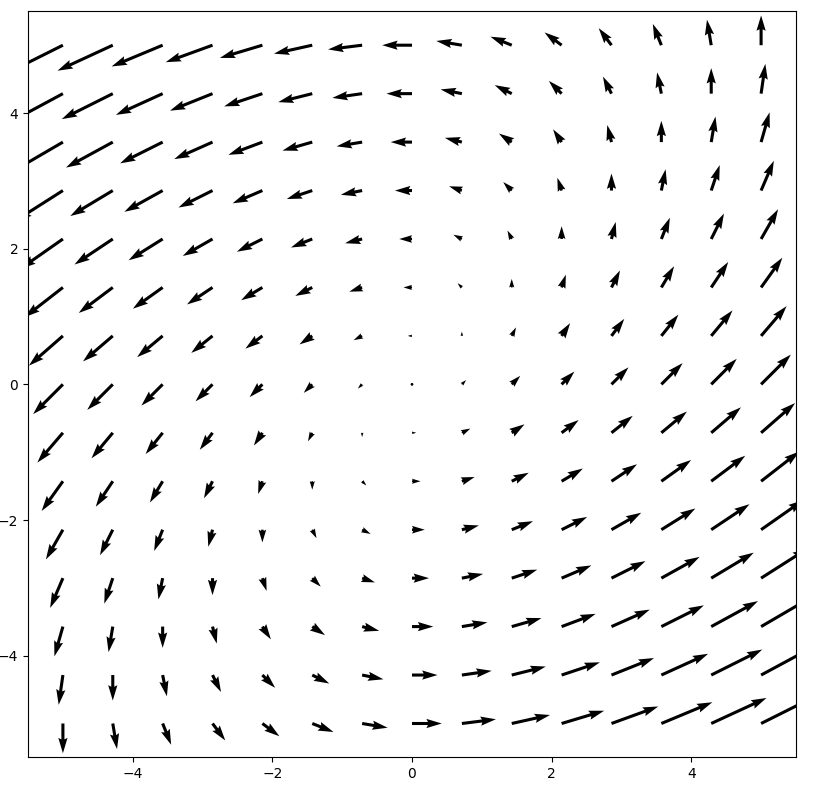
\includegraphics[scale=0.28]{fig2.png}

\begin{center}Figure I \end{center}
\end{minipage}
\begin{minipage}{0.45\textwidth}
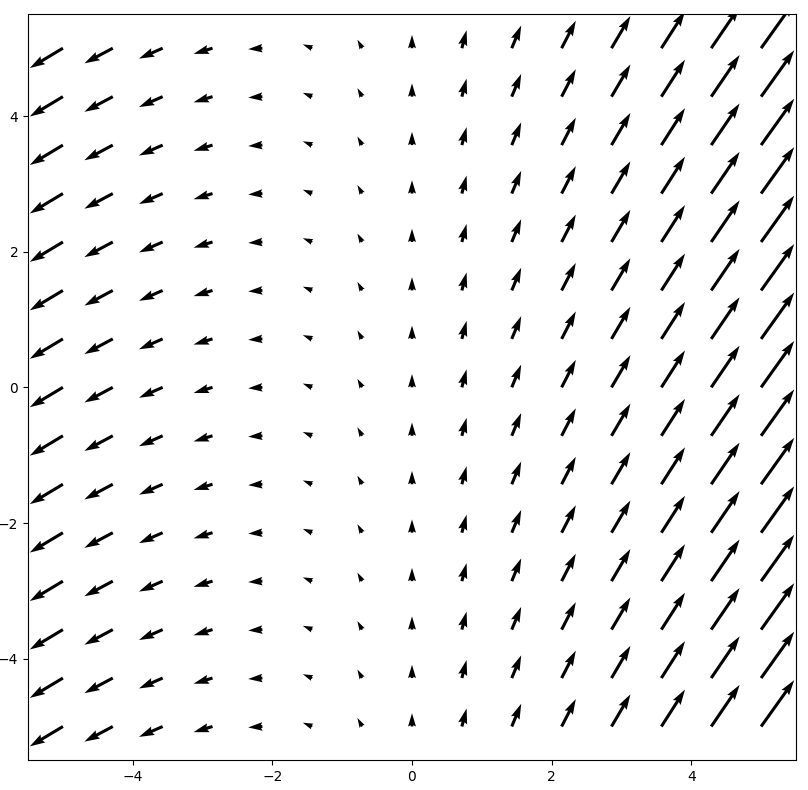
\includegraphics[scale=0.28]{fig1.png}

\begin{center}Figure II \end{center}
\end{minipage}
\end{center}

\part[5] Is it a conservative vector field?
\end{parts}

\newpage

\question
Evaluate the following integrals.
  \begin{parts}
  \part[5] 
  $\displaystyle \int_C x \, ds$, where $C$ is the line segment from $(0, 0)$ to $(2, 4)$. 
  \part[5]
  $\displaystyle \int_C \vec{F} \cdot d \vec{r}$, where $\vec{F} (x, y) = \left\langle xy^2 , -x^2 \right\rangle$ and $\vec{r} (t) = \left\langle t^3 , t^2 \right\rangle$, $0 \leq t \leq 1$. 
  \end{parts}

\newpage

\question[10]
Consider the following vector field:
  \[
    \vec{F} (x, y) = \left\langle 2x y + \frac{y^3}{3} , x^2 + xy^2 \right\rangle .
  \]
\begin{enumerate}[label=(\alph*)]
  \item Is $\vec{F}$ conservative? If so, find a function $f$ such that $\vec{\nabla} f = \vec{F}$.
  \item Evaluate the integral
    \[
       \int_C \vec{F} \cdot d \vec{r}
     \] 
  along the path $C$ parametrized by $\vec{r} (t) = \left\langle \big( \tfrac{t}{\pi} \big)^2 - \sin (t) , \tfrac{t}{\pi} + \big( \frac{t}{\pi} \big)^2 \cos (t + \pi ) \right\rangle$, where $0 \leq t \leq \pi$.
\end{enumerate}

\newpage

\question[10]
Evaluate the integral
  \[
    \int_C (y \cos x - xy \sin x) \, dx + (xy + x \cos x) \, dy ,
  \]
where $C$ is the rectangle with vertices $(0, 0)$, $(0, 4)$, $(2, 4)$ and $(2, 0)$. 

\newpage

\rule{0.3\textwidth}{.4pt} \hspace*{0.2cm} \begin{large}{\textsc{Bonus Question}} \end{large} \hspace*{0.2cm} \hrulefill 

Let $C$ be a closed path surrounding the origin and parametrized by $\vec{r} (t)$. Let $\vec{F}$ be the vector field
  \[
    \vec{F} (x ,y) = \left\langle \frac{-y}{x^2 + y^2}, \frac{x}{x^2 + y^2} \right\rangle .
  \]
What is the value of $\displaystyle \int_C \vec{F} \cdot d \vec{r}$ ?

\end{questions}

\end{document}